\documentclass{article}
\usepackage[UTF8]{ctex}

\usepackage{setspace}
\usepackage[colorlinks,linkcolor=blue,anchorcolor=red,citecolor=black]{hyperref}
\usepackage{lineno}
\usepackage{booktabs}
\usepackage{graphicx}
\usepackage{float}
\usepackage{floatrow}
\usepackage{subfigure}
\usepackage{caption}
\usepackage{subcaption}
\usepackage{geometry}
\usepackage{multirow}
\usepackage{longtable}
\usepackage{lscape}
\usepackage{booktabs}
\usepackage{natbib}
\usepackage{natbibspacing}
\usepackage[toc,page]{appendix}
\usepackage{makecell}


\title{写在前面的一些东西, 又名README}
\date{}

\linespread{1.5}
\geometry{left=2cm,right=2cm,top=2cm,bottom=2cm}

\begin{document}

\maketitle

\begin{figure}
  \centering
  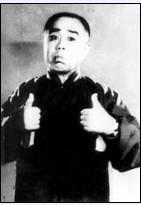
\includegraphics{Figures/刘宝瑞.jpg}
  \caption{相声名家刘宝瑞。大概是在演单口相声《珍珠翡翠白玉汤》的最后一个包袱:文武百官一听这句话,站起来各伸双指,俩大拇哥都挑起来了,可就是没说话。}
\end{figure}
  
  \newpage
  \linenumbers

我记得是在高中语文课本,应该是先秦诸子选读那一本,某一章节最后引清儒论诸子文章,称孟轲、墨翟之文是写给别人看的,故孟子文章雄辩滔滔,墨子文章反复辨难,此皆唯恐读者不明其旨;老聃、庄周之文是写给自己看的,故老子文章言简意赅,庄子文章寓言十九,此皆不以读者为意。
若依此划分,则我这儿的各种东西,便是写给自己看的,不以读者为意也。
\newline
这些东西其实是之前手写的读书笔记。
今欲对其作一整理,各篇皆重新编订。
有些本就是英文写的,我也就如此发出来,不打算做翻译工作。
反正是写给我自己看的。您要是乐意看就看,不乐意就拉倒。
\newline
还有一件事,我是学生物的,但写的东西不一定归哪一科管。
换种思路,学问本无所谓分类。
今天说的文学、哲学、数学、生物学、物理学,以及各种乱七八糟不知所云的学,本就是人强行作的分类。
这事情大概得追溯到亚里士多德那个年月。
总之,既然学问本是一个整体,我一生科狗,写点儿别的东西也不算越界。
只是非科班出身,难入方家法眼。
\newline
还有一件事。
俗话说一千个读者眼里有一千个哈姆雷特,我自己的笔记自然也夹带些私货,从具体内容到内容之编排,多多少少有些个人见解。
这些东西说不上高深,也不一定对。
说不定过几年我就不这么想了,把之前的文章拿出来修修补补也说不定。
在此得说一个人,木心。
这位先生有够机灵的,给人讲文学史,不叫文学史,叫“文学回忆录”。
如此一来,不必纠结于史家论史之客观严谨,可以肆无忌惮地发议论。
罗素在这一点就不够明白。
其本人就是位大哲学家,不乏真知灼见,写西哲史也忍不住议论古人,鲜有史家之风,故其书褒贬不一。
要是罗素也给他的大作起个“西方哲学回忆录”之类的名字,大概其名誉要上涨不少。
我的东西呢,大概也就是这种“回忆录”性质。
当然,我没木心和罗素那么大学问。
人家的想法写出来叫“观点”、“看法”、“评论”,我的顶多叫“偏见”、“瞎掰”、“扯淡”。
\newline
最后一件事,写篇东西还挺费功夫的。
每天晚上对着电脑搜肠刮肚才得二三百字,又要斟酌。
有时候写着写着蟑螂爬桌子上了,还得找本大部头拍它。
日更不太现实,我争取以月更为目标吧。
\newline
以上    

\end{document}